\documentclass[12pt, a4paper, oneside]{ctexart}
\usepackage{amsmath, amsthm, amssymb, bm, color, graphicx, geometry, hyperref, mathrsfs,extarrows, braket, booktabs, array}

\linespread{1.5}
%\geometry{left=2.54cm,right=2.54cm,top=3.18cm,bottom=3.18cm}
\geometry{left=1.84cm,right=1.84cm,top=2.18cm,bottom=2.18cm}
\newenvironment{problem}{\par\noindent\textbf{题目. }}{\bigskip\par}
\newenvironment{solution}{\par\noindent\textbf{解答. }}{\bigskip\par}
\newenvironment{note}{\par\noindent\textbf{注记. }}{\bigskip\par}

% 基本信息
\newcommand{\RQ}{\today} % 日期
\newcommand{\km}{复变函数} % 科目
\newcommand{\bj}{强基数学002} % 班级
\newcommand{\xm}{吴天阳} % 姓名
\newcommand{\xh}{2204210460} % 学号

\begin{document}

%\pagestyle{empty}
\pagestyle{plain}
\vspace*{-15ex}
\centerline{\begin{tabular}{*5{c}}
    \parbox[t]{0.25\linewidth}{\begin{center}\textbf{日期}\\ \large \textcolor{blue}{\RQ}\end{center}} 
    & \parbox[t]{0.2\linewidth}{\begin{center}\textbf{科目}\\ \large \textcolor{blue}{\km}\end{center}}
    & \parbox[t]{0.2\linewidth}{\begin{center}\textbf{班级}\\ \large \textcolor{blue}{\bj}\end{center}}
    & \parbox[t]{0.1\linewidth}{\begin{center}\textbf{姓名}\\ \large \textcolor{blue}{\xm}\end{center}}
    & \parbox[t]{0.15\linewidth}{\begin{center}\textbf{学号}\\ \large \textcolor{blue}{\xh}\end{center}} \\ \hline
\end{tabular}}
\vspace*{4ex}
\def\disp{\displaystyle}
% 正文部分
\paragraph{习题\ 第四章}
\paragraph{1.}计算积分

(1)$\disp\int_{|z| = 2}\frac{e^z}{1+z^2}\,dz;$\qquad\qquad\qquad(2)$\disp\int_{|z+i|=1}\frac{e^z}{1+z^2}\,dz$
\begin{solution}
    \begin{equation*}
        (1)\quad\int_{|z| = 2}\frac{e^z}{1+z^2}\,dz = \frac{1}{2i}\int_{|z| = 2}e^z\left(\frac{1}{z-i}-\frac{1}{z+i}\right)\,dz\xlongequal{\text{Cauchy公式}}\pi(e^i-e^{-i}) = 2\pi i\sin1
    \end{equation*}
    \begin{equation*}
        \begin{aligned}
            (2)\quad\int_{|z+i| = 1}\frac{e^z}{1+z^2}\,dz = \frac{1}{2i}\int_{|z+i|=1}e^z\left(\frac{1}{z-i}-\frac{1}{z+i}\right)\,dz\xlongequal{\text{Cauchy定理}}&\ \frac{1}{2\pi}\int_{|z+i|=1}-\frac{e^z}{z+i}\,dz\\
            \xlongequal{\text{Cauchy公式}}&\ -\pi e^{-i}
        \end{aligned}
    \end{equation*}
\end{solution}
\paragraph{2.}计算积分
(1)$\disp \int_{|z| = 2}\frac{dz}{(z-1)^3(z-3)^3};$
(2)$\disp \int_{|z| = R}\frac{dz}{(z-a)^n(z-b)},a,b\text{不在圆周}|z| = R\text{上},n\in\mathbb{N}.$
\begin{solution}
    \begin{equation*}
        (1)\quad \int_{|z| = 2}\frac{dz}{(z-1)^3(z-3)^3} \xlongequal{\text{Cauchy公式}}\frac{2\pi i}{2!}\left(\frac{1}{(z-3)^3}\right)^{(2)}\biggl|_{z=1}=\pi i\cdot \frac{12}{(-2)^5} = -\frac{3\pi i}{8}
    \end{equation*}
    (2) 若$a, b$均在$|z|<R$的圆内或圆外,由Cauchy定理可知,$\disp \int_{|z| = R}\frac{dz}{(z-a)^n(z-b)} = 0$;若$a$在圆内,$b$在圆外,则
    \begin{equation*}
      \disp \int_{|z| = R}\frac{dz}{(z-a)^n(z-b)} \xlongequal{\text{Cauchy公式}}\frac{2\pi i}{(n-1)!}\left(\frac{1}{z-b}\right)^{(n-1)}\biggl|_{z=a} = (-1)^{n-1}\frac{2\pi i}{(a-b)^n} = -\frac{2\pi i}{(b-a)^n}  
    \end{equation*}
    若$b$在圆内,$a$在圆外,则$\disp \int_{|z| = R}\frac{dz}{(z-a)^n(z-b)} \xlongequal{\text{Cauchy公式}}\frac{2\pi i}{(b-a)^n}$。
\end{solution}
\paragraph{3.}计算积分 \begin{equation*}
    \begin{aligned}
        (1)&\ \int_{|z| = 2}\bar{z}\,dz;\qquad\qquad(2) \int_{|z| = 2}\frac{|dz|}{z-1};\\
        (3)&\ \int_{|z| = 1}\frac{\bar{z}^kP_n(z)}{z-z_0}\,dz,|z_0|<1,0\leqslant k\leqslant n,P_n(z) = a_0+a_1z+\cdots+a_nz^n.
    \end{aligned}
\end{equation*}
\begin{solution}
    (1) 令$\gamma(\theta) = 2e^{i\theta}$,则$\disp\int_{|z| = 2}\bar{z}\,dz = \int_0^\pi 2e^{-i\theta}2ie^{i\theta}\,d\theta = 8\pi i$

    (2) 令$\gamma(\theta) = 2e^{i\theta}$,则$|dz| = 2\,d\theta$,于是$dz = 2ie^{i\theta}\,d\theta=\dfrac{iz|dz|}{2}$,所以
    \begin{equation*}
        \int_{|z| = 2}\frac{|dz|}{z-1} = \int_{|z| = 2}\frac{2\,dz}{i(z-1)z} \xlongequal{\text{Cauchy定理}} 0
    \end{equation*}

    \begin{equation*}
        \begin{aligned}
            (3)\quad\int_{|z| = 1}\frac{\bar{z}^kP_n(z)}{z-z_0}\,dz =&\ \int_{|z| = 1}\frac{P_n(z)}{z^k(z-z_0)}\,dz=\int_{|z| = 1}\frac{\sum_{j=0}^{k-1}a_jz^j}{z^k(z-z_0)}\,dz+\int_{|z| = 1}\frac{\sum_{j=k}^na_jz^j}{z^k(z-z_0)}\\
            \xlongequal{\text{Cauchy定理}}&\ \int_{|z| = 1}\frac{\sum_{j=k}^na_jz^{j-k}}{z-z_0}\xlongequal{\text{Cauchy公式}}2\pi i\sum_{j=k}^na_jz_0^{j-k}
        \end{aligned}
    \end{equation*}
\end{solution}
\paragraph{5.}计算积分\begin{equation*}
    \frac{1}{2\pi i}\int_{|z| = R}\frac{z+a}{z-a}\,\frac{dz}{z}\quad(|a| < R)
\end{equation*}
求证\begin{equation*}
    \frac{1}{2\pi}\int_0^{2\pi}\frac{R^2-|a|^2}{|z-a|^2}\,d\theta = 1\quad(z = Re^{i\theta})
\end{equation*}
\begin{solution}
    \begin{equation*}
        \frac{1}{2\pi i}\int_{|z| =R}\frac{z+a}{z-a}\,\frac{dz}{z} = \frac{1}{2\pi i}\int_{|z| = R}\left(\frac{2}{z-a}-\frac{1}{z}\right)\,dz\xlongequal{\text{Cauchy公式}}2-1 = 1
    \end{equation*}
    由上式可知
    \begin{equation*}
        \begin{aligned}
            1 =&\ \frac{1}{2\pi i} \int_{|z| = R}\frac{(z+a)\,dz}{(z-a)z}=\frac{1}{2\pi i}\int_{|z| = R} \frac{(z+a)(\bar{z}-\bar{a})\,dz}{|z-a|^2z}=\frac{1}{2\pi i}\int_{|z| = R}\frac{|z|^2-|a|^2-z\bar{a}+a\bar{z}}{|z-a|^2z}\,dz\\
            \xlongequal{\text{Cauchy定理}}&\ \frac{1}{2\pi i}\int_{|z| = R}\frac{|z|^2-|a|^2}{|z-a|^2z}\,dz \xlongequal{z = Re^{i\theta}}\frac{1}{2\pi}\int_0^{2\pi}\frac{R^2-|a|^2}{|z-a|^2}\,d\theta
        \end{aligned}
    \end{equation*}
\end{solution}
\paragraph{7.}设$f(z)$在$\mathbb{C}$上解析,且当$z\rightarrow \infty$时,$|f(z)| = O(|z|^k)(k > 0)$。证明:$f(z)$是一次数$\leqslant k$的多项式。
\begin{proof}
    由于$f(z)$为整函数,对于充分大的$R$,$\exists M$使得$|f(R)| = M\cdot R^k$,由Cauchy公式可知
    \begin{equation*}
        |f^{(k+1)}(z)| = \left|\frac{(k+1)}{2\pi i}\int_{|z| = R}\frac{f(\xi)}{(\xi - z)^{k+2}}\,d\xi \right|\leqslant \frac{(k+1)!}{2\pi}\cdot \frac{M\cdot R^k}{(R-|z|)^{k+2}}\cdot 2\pi R
    \end{equation*}
    当$R\rightarrow \infty$时,$|f^{(k+1)}(z)| = 0$,则$f(z)$是次数$\leqslant k$的多项式。
\end{proof}
\paragraph{8.}试用Liouville定理证明每一多项式$P(z)$至少有一零点。
\begin{proof}
    反设$P(z)$在$\mathbb{C}$上没有零点,由于$|P(z)|$一定存在下界$m > 0$上界$\infty$,则$\frac{1}{P(z)}$有界,即$|\frac{1}{P(z)}|\leqslant \frac{1}{m} < \infty$,由Liouville定理可知,$\frac{1}{P(z)}$为常值函数,与$P(x)$为多项式矛盾,所以多项式$P(x)$至少有一零点。
\end{proof}
\paragraph{10.}若非常数函数$f(z)$在$1<|z|<+\infty$内解析,且$\disp\lim_{z\rightarrow \infty}f(z)=f(\infty)$存在,证明:

(1) $\disp f(\infty) = \frac{1}{2\pi}\int_0^{2\pi}f(Re^{i\theta})\,d\theta,\ R > 1;$

(2) 在$|z|>1$上最大模原理成立。
\begin{proof}
    \begin{equation*}
        \begin{aligned}
            (1)\quad\frac{1}{2\pi}\int_0^{2\pi}f(Re^{i\theta})\,d\theta-f(\infty) =&\ \frac{1}{2\pi}\int_0^{2\pi}(f(Re^{i\theta})-f(\infty))\,d\theta = \frac{1}{2\pi i}\int_{|z| = R}\frac{f(z)-f(\infty)}{z}\,dz\\
            \xlongequal[\text{Cauchy定理}]{\text{充分大的} R_1}&\ \frac{1}{2\pi i}\int_{|z| = R_1}\frac{f(z)-f(\infty)}{z}\,dz\leqslant |f(R_1e^{i\theta})-f(\infty)|\rightarrow 0
        \end{aligned}
    \end{equation*}
    所以$\disp f(\infty) = \frac{1}{2\pi}\int_0^{2\pi}f(Re^{i\theta})\,d\theta,\ R > 1$

    (2) 只需证明最大模原理在$f(\infty)$处成立即可,设$\disp M = \lim_{1<|z|<\infty}$,由(1)可知\begin{equation*}
        f(\infty) = \frac{1}{2\pi}\int_0^{2\pi}f(Re^{i\theta})\,d\theta \leqslant |f(Re^{i\theta})| < M
    \end{equation*}
    所以最大模原理在$f(\infty)$处同样成立,故在$|z|>1$上最大模原理成立。
\end{proof}
\paragraph{14.}设函数$f(z)$在园$|z|<R$内解析,且$|f(z)|\leqslant M,f(0) = 0$。证明:
\begin{equation*}
    |f(z)|\leqslant \frac{M}{R}|z|,\quad|f'(0)|\leqslant \frac{M}{R},
\end{equation*}
其中等号仅当$\disp f(z)=\frac{M}{R}e^{i\alpha}z$($\alpha$为实数)时才成立。
\begin{proof}
    设$\disp \varphi(z)=\begin{cases}
        \frac{f(z)}{z},\quad&0 <|z|<R,\\
        f'(0),\quad&|z| = 0.
    \end{cases}$,类比Schwarz引理可证得$\varphi(z)$在$|z| < R$内解析,对于$\forall z_0 < R$,$\exists |z_0| < r < R$,则\begin{equation*}
        |\varphi(z_0)|\leqslant \max_{|z|=r}\left|\frac{f(z)}{z}\right|\leqslant \frac{M}{r}
    \end{equation*}
    令$r\rightarrow R$得,且$z_0$具有任意性可知,$|\varphi(z)|\leqslant \frac{M}{R}$,所以$ |f(z)|\leqslant \frac{M}{R}|z|$和$|f'(0)|\leqslant \frac{M}{R}$。当取到等号时,即$\exists |z_0|<R$,使得$\varphi(z_0)=\frac{M}{R}$,由最大模原理可知,$|\varphi(z)|\equiv \frac{M}{R}$,故$\varphi(z) = \frac{M}{R}e^{i\theta}$,所以$ f(z)=\frac{M}{R}e^{i\theta}z\ (\theta\in \mathbb{R})$。
\end{proof}
\paragraph{20.}设$P_n(z)$为$n$次多项式,$|z|\leqslant 1$时,$|P_n(z)|\leqslant M$。证明:$|z|\leqslant 1$时,$|P'(z)|\leqslant enM.$
\begin{proof}
    由Cauchy公式可知,对$|z| \leqslant R(R> 1)$时,有
    \begin{equation*}
        \begin{aligned}
            |P'(z)| =&\ \left|\frac{1}{2\pi i}\int_{|z| = R}\frac{P_n(\xi)}{(\xi-z)^2}\,d\xi\right|\leqslant \frac{1}{2\pi}\int_{|z|=R}\frac{|P_n(\xi)}{|\xi-z|^2}|d\xi|\\
            \leqslant&\ \frac{MR^n}{2\pi}\int_0^{2\pi}\frac{R\,d\theta}{|\xi-z|^2}\quad(\text{由11题可知})\\
            \leqslant&\ \frac{MR^n}{2\pi}\cdot\frac{R\cdot 2\pi}{|R|^2-|z|^2}\leqslant \frac{MR^{n+1}}{R^2-1}\quad(\text{三角不等式})
        \end{aligned}
    \end{equation*}
    令$n = \dfrac{1}{R^2-1}$,即$R = \sqrt{1+\dfrac{1}{n}}$,则
    \begin{equation*}
        |P'(z)|\leqslant nM\left(1+\frac{1}{n}\right)^{\frac{n+1}{2}} \leqslant nM\left(1+\frac{1}{n}\right)^n\leqslant enM\quad(\text{由于}\left(1+\frac{1}{n}\right)^2\text{为增函数})
    \end{equation*}
\end{proof}


% 下面给一些功能的写法
\iffalse
% 图片模板
\centerline{
    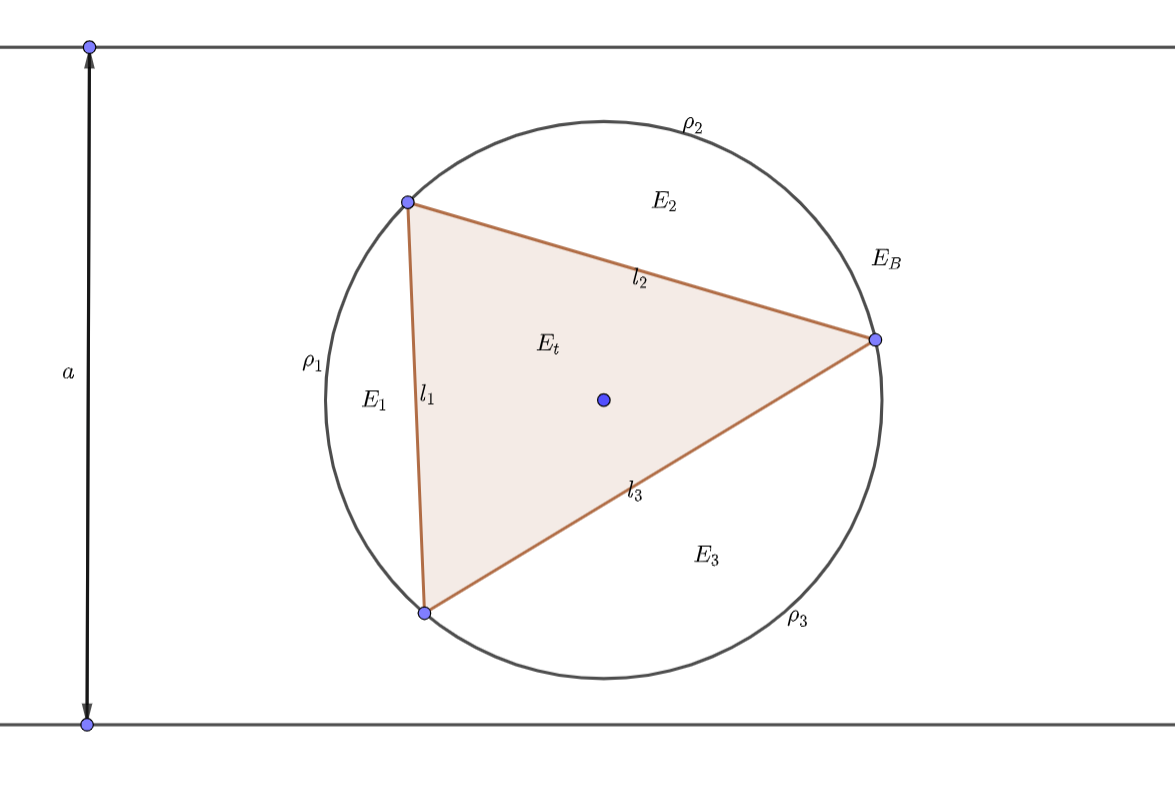
\includegraphics[width=0.8\textwidth]{figure.png}
}
% 表格模板
\renewcommand\arraystretch{0.8} % 设置表格高度为原来的0.8倍
\begin{table}[!htbp] % table标准
    \centering % 表格居中
    \begin{tabular}{p{1cm}<{\centering}p{1cm}<{\centering}p{3cm}<{\centering}p{5cm}<{\centering}} % 设置表格宽度
    %\begin{tabular}{cccc}
        \toprule
        $x_i$ & $f[x_1]$ & $f[x_i,x_{i+1}]$ & $f[x_i,x_{i+1},x_{i+2}]$ \\
        \midrule
        $x_0$ & $f(x_0)$ &                  &                          \\
        $x_0$ & $f(x_0)$ & $f'(x_0)$        &                          \\
        $x_0$ & $f(x_1)$ & $\frac{f(x_1)-f(x_0)}{x_1-x_0}$ & $\frac{f(x_1)-f(x_0)}{(x_1-x_0)^2}-\frac{f'(x_0)}{x_1-x_0}$\\
        \bottomrule
    \end{tabular}
\end{table}

\def\Log{\text{Log}} % 一个简单的宏定义
$\Log$ % 调用方法
\fi

\end{document}